\documentclass[9pt,lineno]{elife}

% graphicx package, useful for including eps and pdf graphics
\usepackage{graphicx}
\DeclareGraphicsExtensions{.png,.png,.jpg}

% basic packages
\usepackage{color}
\usepackage{parskip}
\usepackage{float}
\usepackage{microtype}
\usepackage{url}
\usepackage{hyperref}
\usepackage{booktabs}
\usepackage{makecell}
\usepackage{multirow}

% text layout
\usepackage{geometry}
\geometry{textwidth=17cm} % 15.25cm for single-space, 16.25cm for double-space
\geometry{textheight=22.5cm} % 22cm for single-space, 22.5cm for double-space

% helps to keep figures from being orphaned on a page by themselves
\renewcommand{\topfraction}{0.85}
\renewcommand{\textfraction}{0.1}

% bold the 'Figure #' in the caption and separate it with a period
% Captions will be left justified
\usepackage[labelfont=bf,labelsep=period,font=small]{caption}

% cite package, to clean up citations in the main text. Do not remove.
%\usepackage{cite}
%\usepackage{natbib}

%% \usepackage{lineno}
%% \linenumbers

\usepackage{authblk}
\renewcommand\Authands{ \& }
\renewcommand\Authfont{\normalsize \bf}
\renewcommand\Affilfont{\small \normalfont}
\makeatletter
\renewcommand\AB@affilsepx{, \protect\Affilfont}
\makeatother

% latexdiff

%DIF UNDERLINE PREAMBLE %DIF PREAMBLE
\RequirePackage[normalem]{ulem} %DIF PREAMBLE
\RequirePackage{color}\definecolor{RED}{rgb}{1,0,0}\definecolor{BLUE}{rgb}{0,0,1} %DIF PREAMBLE
\providecommand{\DIFadd}[1]{{\protect\color{blue}\uwave{#1}}} %DIF PREAMBLE
\providecommand{\DIFdel}[1]{{\protect\color{red}\sout{#1}}}                      %DIF PREAMBLE
%DIF SAFE PREAMBLE %DIF PREAMBLE
\providecommand{\DIFaddbegin}{} %DIF PREAMBLE
\providecommand{\DIFaddend}{} %DIF PREAMBLE
\providecommand{\DIFdelbegin}{} %DIF PREAMBLE
\providecommand{\DIFdelend}{} %DIF PREAMBLE
%DIF FLOATSAFE PREAMBLE %DIF PREAMBLE
\providecommand{\DIFaddFL}[1]{\DIFadd{#1}} %DIF PREAMBLE
\providecommand{\DIFdelFL}[1]{\DIFdel{#1}} %DIF PREAMBLE
\providecommand{\DIFaddbeginFL}{} %DIF PREAMBLE
\providecommand{\DIFaddendFL}{} %DIF PREAMBLE
\providecommand{\DIFdelbeginFL}{} %DIF PREAMBLE
\providecommand{\DIFdelendFL}{} %DIF PREAMBLE

% comments
%% \definecolor{purple}{rgb}{0.459,0.109,0.538}
%% \def\tbc#1{\textcolor{purple}{[#1]}}
%% \def\rnc#1{\textcolor{blue}{[#1]}}
\def\jhc#1{\textcolor{red}{[#1]}}

\title{Genetic cartography reveals ancestral relationships of human pathogenic viruses}

\author[1]{Sravani Nanduri}
\author[2]{Allison Black}
\author[2,3]{Trevor Bedford}
\author[2*]{John Huddleston}

\affil[1]{Paul G. Allen School of Computer Science and Engineering, University of Washington, Seattle, WA, USA}
\affil[2]{Vaccine and Infectious Disease Division, Fred Hutchinson Cancer Research Center, Seattle, WA, USA}
\affil[3]{Howard Hughes Medical Institute, Seattle, WA, USA}

\corr{jhuddles@fredhutch.org}{JH}

\date{}

\begin{document}
\maketitle

\begin{abstract}
\end{abstract}

\section*{Introduction}

Tracking the evolution of human pathogenic viruses in real time enables epidemiologists to respond quickly to emerging epidemics and local outbreaks.
Real-time analyses of viral evolution typically rely on phylogenetic methods.
These methods can reconstruct the evolutionary history of viral populations from their genome sequences and estimate states of inferred ancestral viruses including their most likely genome sequence, time of circulation, and geographic location (gen epi papers).
Importantly, these methods assume that all sequence data share an evolutionary history represented by the clonal replication of genomes.
In practice, the evolutionary histories of many human pathogenic viruses including seasonal influenza viruses, Zika virus, and coronaviruses violate this assumption through processes of reassortment or recombination.
Researchers have attempted to compensate for these evolutionary mechanisms by limiting their analyses to specific genes (citation?), concatenating multiple genes despite their different evolutionary histories (citation?), or developing more sophisticated models to represent the joint likelihoods of multiple co-evolving lineages represented by networks rather than trees (Muller).
However, several key questions in genomic epidemiology do not require full phylogenetic inference of ancestral relationships and states.
For example, genomic epidemiologists commonly need to 1) identify clusters of closely-related genomes that represent regional outbreaks or new variants of concern (Black et al.? MicrobeTrace?), 2) rapidly place newly sequenced viral genomes in the evolutionary context of other circulating strains (USHER, NextClade), and 3) flag low-quality or mislabeled genome sequences for exclusion from their analyses.
These common use cases can all be addressed by standard statistical methods including clustering, classification, and outlier detection.
These methods make few assumptions about the input data and therefore should be applicable to genomic data that violate phylogenetic assumptions.

To apply these methods to a population of viral genomes, we need metrics to compare genome sequences to each other and algorithms to reduce the highly multidimensional input data ($M \times N$ values for $M$ genomes of length $N$) to one or two dimensions where clustering, classification, and outlier detection are more tractable.
The number of mismatches between any pair of aligned genome sequences, also known as the Hamming distance, provides a natural distance metric for viral genomes.
Indeed, most phylogenetic methods start by building a matrix of Hamming distances between all sequences in a given multiple sequence alignment.
Many dimensionality reduction algorithms including multidimensional scaling (MDS) \citep{hout_papesh_goldinger_2012}, t-SNE \citep{maaten2008visualizing}, and UMAP \citep{lel2018umap} accept such distance matrices as an input and produce a corresponding lower-dimensional representation or “embedding” of those data.
Alternately, principal components analysis (PCA) only requires the input data to be transformed to a matrix of integers before it can embed those data into a few orthogonal dimensions.

Each of these embedding methods has been applied to genomic data to visualize relationships between individuals and identify clusters of related genomes.
Although PCA is a generic linear algebra algorithm that optimizes for an orthogonal embedding of the data, the principal components from single nucleotide polymorphisms (SNPs) represent mean coalescent times and therefore recapitulate broad phylogenetic relationships \citep{mcvean_2009}.
PCA has been applied to SNPs of human genomes \citep{novembre_2008,alexander_2009,mcvean_2009,auton_2015} and to multiple sequence alignments of viral genomes \citep{metsky_2017}.
MDS attempts to embed input data into a lower-dimensional representation such that each pair of data points are as far apart in the embedding as they are in the original data.
MDS has been applied to multiple gene segments of seasonal influenza viruses to visualize evolutionary relationships between segments \citep{rambaut_2008}.
Both t-SNE and UMAP build on manifold learning methods like MDS to find low-dimensional embeddings of data that place similar points close together and dissimilar points far apart \citep{kobak_2021}.
These methods have been applied to SNPs from human genomes \citep{diaz-papkovich_2019} and single-cell transcriptomes \citep{becht_2018,kobak_2019}.

Although these embedding methods are commonly used for qualitative studies of evolutionary relationships, few studies have attempted to quantify patterns observed in these embeddings and no studies have investigated the value of applying these methods to human pathogenic viruses.
To this end, we applied PCA, MDS, t-SNE, and UMAP to genomes from recent populations of seasonal influenza virus A/H3N2, Zika virus, MERS-CoV, and SARS-CoV-2.
Each of these viruses have impacted human populations globally in the last decade and have been studied in real time by genomic epidemiologists.
For each virus and embedding method, we quantified the relationship between pairwise sequence and embedding distances, identified clusters of closely-related genomes in embedding space, and evaluated the accuracy of clusters compared to expert-defined phylogenetic clades.
Finally, we tested the practical application of these methods to identify reassortment and outliers in seasonal influenza viruses.
These results inform our recommendations for future applications of these methods including which methods are most effective for specific problems in genomic epidemiology and which parameters researchers should use for each method.

\section*{Results}

\begin{table}[htb]
  \begin{center}
    \scalebox{0.95}{
      \begin{tabular}{llrr}
\toprule
                     Pathogen & Method &   VI &  Threshold \\
\midrule
               Influenza H3N2 &  t-SNE & 0.04 &        2.0 \\
                              &   UMAP & 0.08 &        1.0 \\
                              &    MDS & 0.10 &        3.5 \\
                              &    PCA & 0.19 &        0.5 \\
SARS-CoV-2 (Nextstrain clade) &  t-SNE & 0.07 &        1.0 \\
                              &    MDS & 0.15 &        0.0 \\
                              &   UMAP & 0.16 &        0.5 \\
                              &    PCA & 0.22 &        0.5 \\
           SARS-CoV-2 (Pango) &  t-SNE & 0.12 &        1.0 \\
                              &    MDS & 0.23 &        0.0 \\
                              &   UMAP & 0.25 &        0.5 \\
                              &    PCA & 0.31 &        0.5 \\
\bottomrule
\end{tabular}

    }
    \caption{
      Accuracy of embedding methods per human pathogenic virus sorted by Matthew's correlation coefficient (MCC).
      The corresponding contingency matrix values for true positives (TP), true negatives (TN), false positives (FP), and false negatives (FN) are also included.
      Threshold refers to the distance threshold used to assign clusters with HDBSCAN.
    }
    \label{table_accuracy}
  \end{center}
\end{table}

\subsection*{Embedding clusters recapitulate phylogenetic clades for seasonal influenza A/H3N2}

Seasonal influenza A/H3N2's hemagglutinin (HA) sequences provide an ideal positive control to test dimensionality reduction methods and clustering.
A/H3N2's HA protein evolves rapidly, accumulating amino acid mutations that enable escape from adaptive immunity in human populations \citep{flu-review}.
These mutations produce distinct phylogenetic clades that represent potentially different antigenic phenotypes.
The World Health Organization (WHO) Global Influenza Surveillance and Response System (GISRS) regularly sequences genomes of circulating influenza lineages \citep{who-gisrs} and submits these sequences to public INSDC databases like NCBI's GenBank \citep{insdc}.
These factors, coupled with HA's relatively short gene size of 1,701 nucleotides, facilitate real-time genomic epidemiology of A/H3N2 \citep{nextflu,nextstrain} and rapid analysis by the embedding methods we wanted to evaluate.

We identified \jhc{NNN} A/H3N2 HA sequences from NCBI's GenBank database (methods) spanning from January 2016 to January 2020.
To evaluate the optimal parameters for each embedding method and avoid overfitting to specific datasets, we partitioned these data into a training dataset from 2016--2018 (N=\jhc{NNN} sequences) and a test dataset from 2018--2020 (N=\jhc{NNN} sequences).
We first analyzed the training data with Nextstrain's seasonal influenza workflow that creates a multiple sequence alignment, infers a time-resolved phylogenetic tree, and assigns clade labels to each sequence based on our own expert-defined clade annotations \citep{nextstrain,seasonal-flu,augur}.
We applied each embedding method to the multiple sequence alignment, identified clusters in the embeddings with HDBSCAN \citep{hdbscan}, and evaluated the accuracy of cluster classifications compared to known clade annotations.
We applied this general approach in an exhaustive grid search to identify the optimal parameters for each combination of embedding method and HDBSCAN (see Methods).

All four embedding methods qualitatively recapitulated clade-level groupings observed in the phylogeny (Figure~\ref{fig:seasonal-influenza-h3n2-ha-embeddings}).
Strains from the same clade generally grouped tightly together in PCA, t-SNE, and UMAP embeddings.
While MDS followed this general pattern, it also produced separate pairs of A3 and A4 clusters that did not correspond to meaningful subclades.
All of the embedding methods clearly delineated larger phylogenetic clades into separate spaces (e.g., A1 and A2) and, with the exception of t-SNE, placed related subclades closer together (e.g., A2 and A2/re or the A1b subclades).
The t-SNE embedding placed distantly related pairs of clades like 3c3.A and A2 as close together as closely-related clades like A2 and its subclade A2/re.
These results suggest that t-SNE maintains both local and global structure, but that our interpretation of the absolute distance between points in these embeddings cannot be linear.

\begin{figure}[htb]
  \begin{center}
  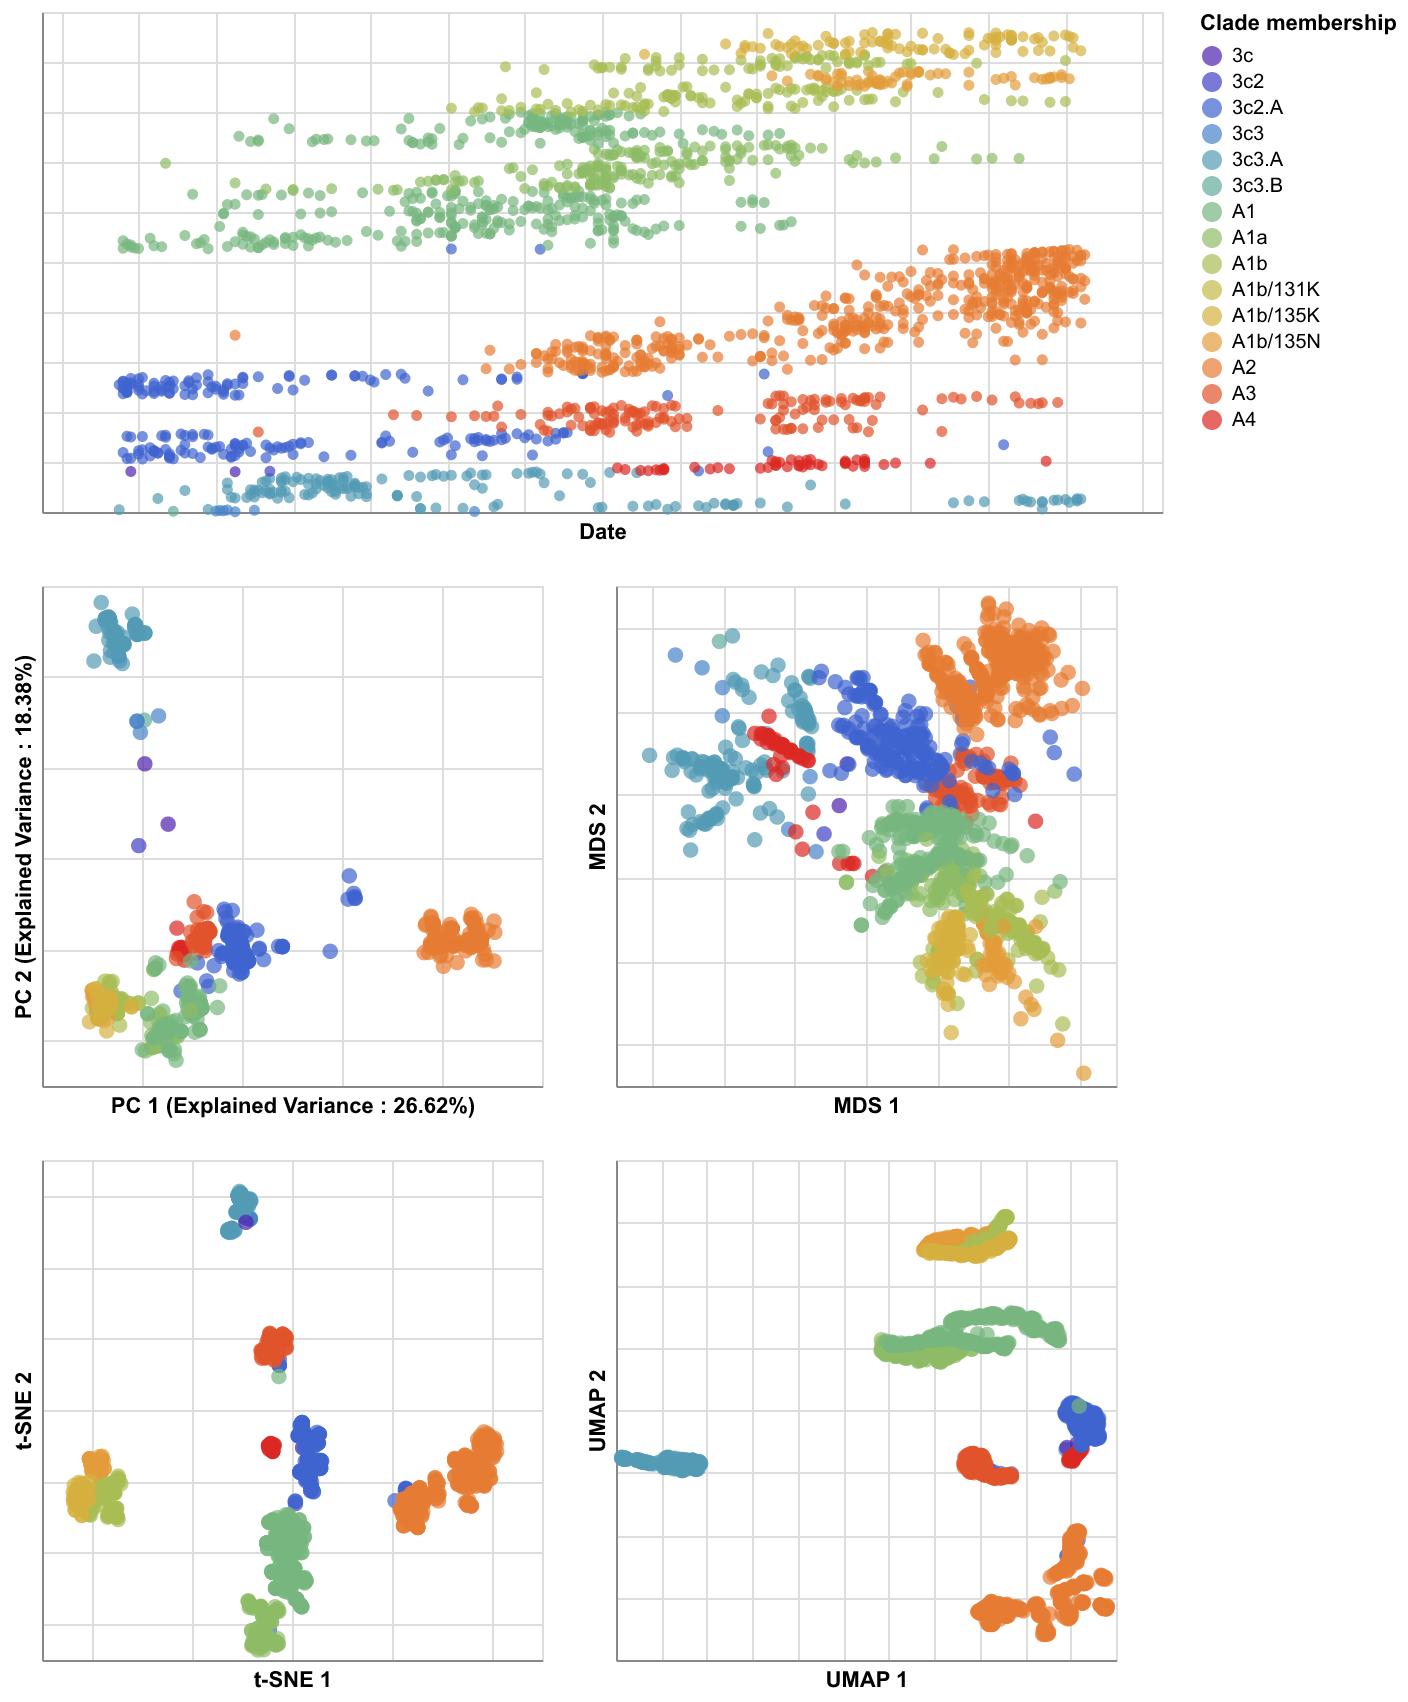
\includegraphics[width=\columnwidth]{figures/flu-2016-2018-ha-embeddings-by-clade.png}
  \caption{
    The phylogeny of influenza A/H3N2 viruses (top) shows the evolutionary relationships among viruses including clades, or viruses that share the same mutations and descend from the same common ancestor.
    Reduced dimensionality embeddings of genetic sequences into two dimensions by PCA (middle left), MDS (middle right), t-SNE (bottom left), and UMAP (bottom right) generally recapitulate groups of viruses into clades without inferring ancestral relationships.
  }
  \label{fig:seasonal-influenza-h3n2-ha-embeddings}
  \end{center}
\end{figure}

To quantify the apparent maintenance of local and global structure in these embeddings, we calculated the relationship between pairwise genetic distance of genomes and pairwise Euclidean distance of those genomes in each embedding.
All four methods maintained a linear relationship between genetic and Euclidean distances for genomes that differed by no more than $\approx$20 nucleotides (Figure~\ref{fig:seasonal-influenza-h3n2-ha-pairwise-distances}).
However, PCA and MDS were the only methods that consistently maintained that linearity as genetic distance increased (Pearson's $R^{2} = 0.767 \pm 0.000$  and $0.849 \pm 0.000$, respectively).
In contrast, the relationship between genetic and Euclidean distance was nonlinear in t-SNE (Pearson's $R^{2} = 0.393 \pm 0.001$) and UMAP (Pearson's $R^{2} = 0.397 \pm 0.000$) embeddings.
Genomes that differed by more than $\approx$20 nucleotides were equally as likely to map close together as far apart in these embeddings.

\begin{figure}[htb]
  \begin{center}
  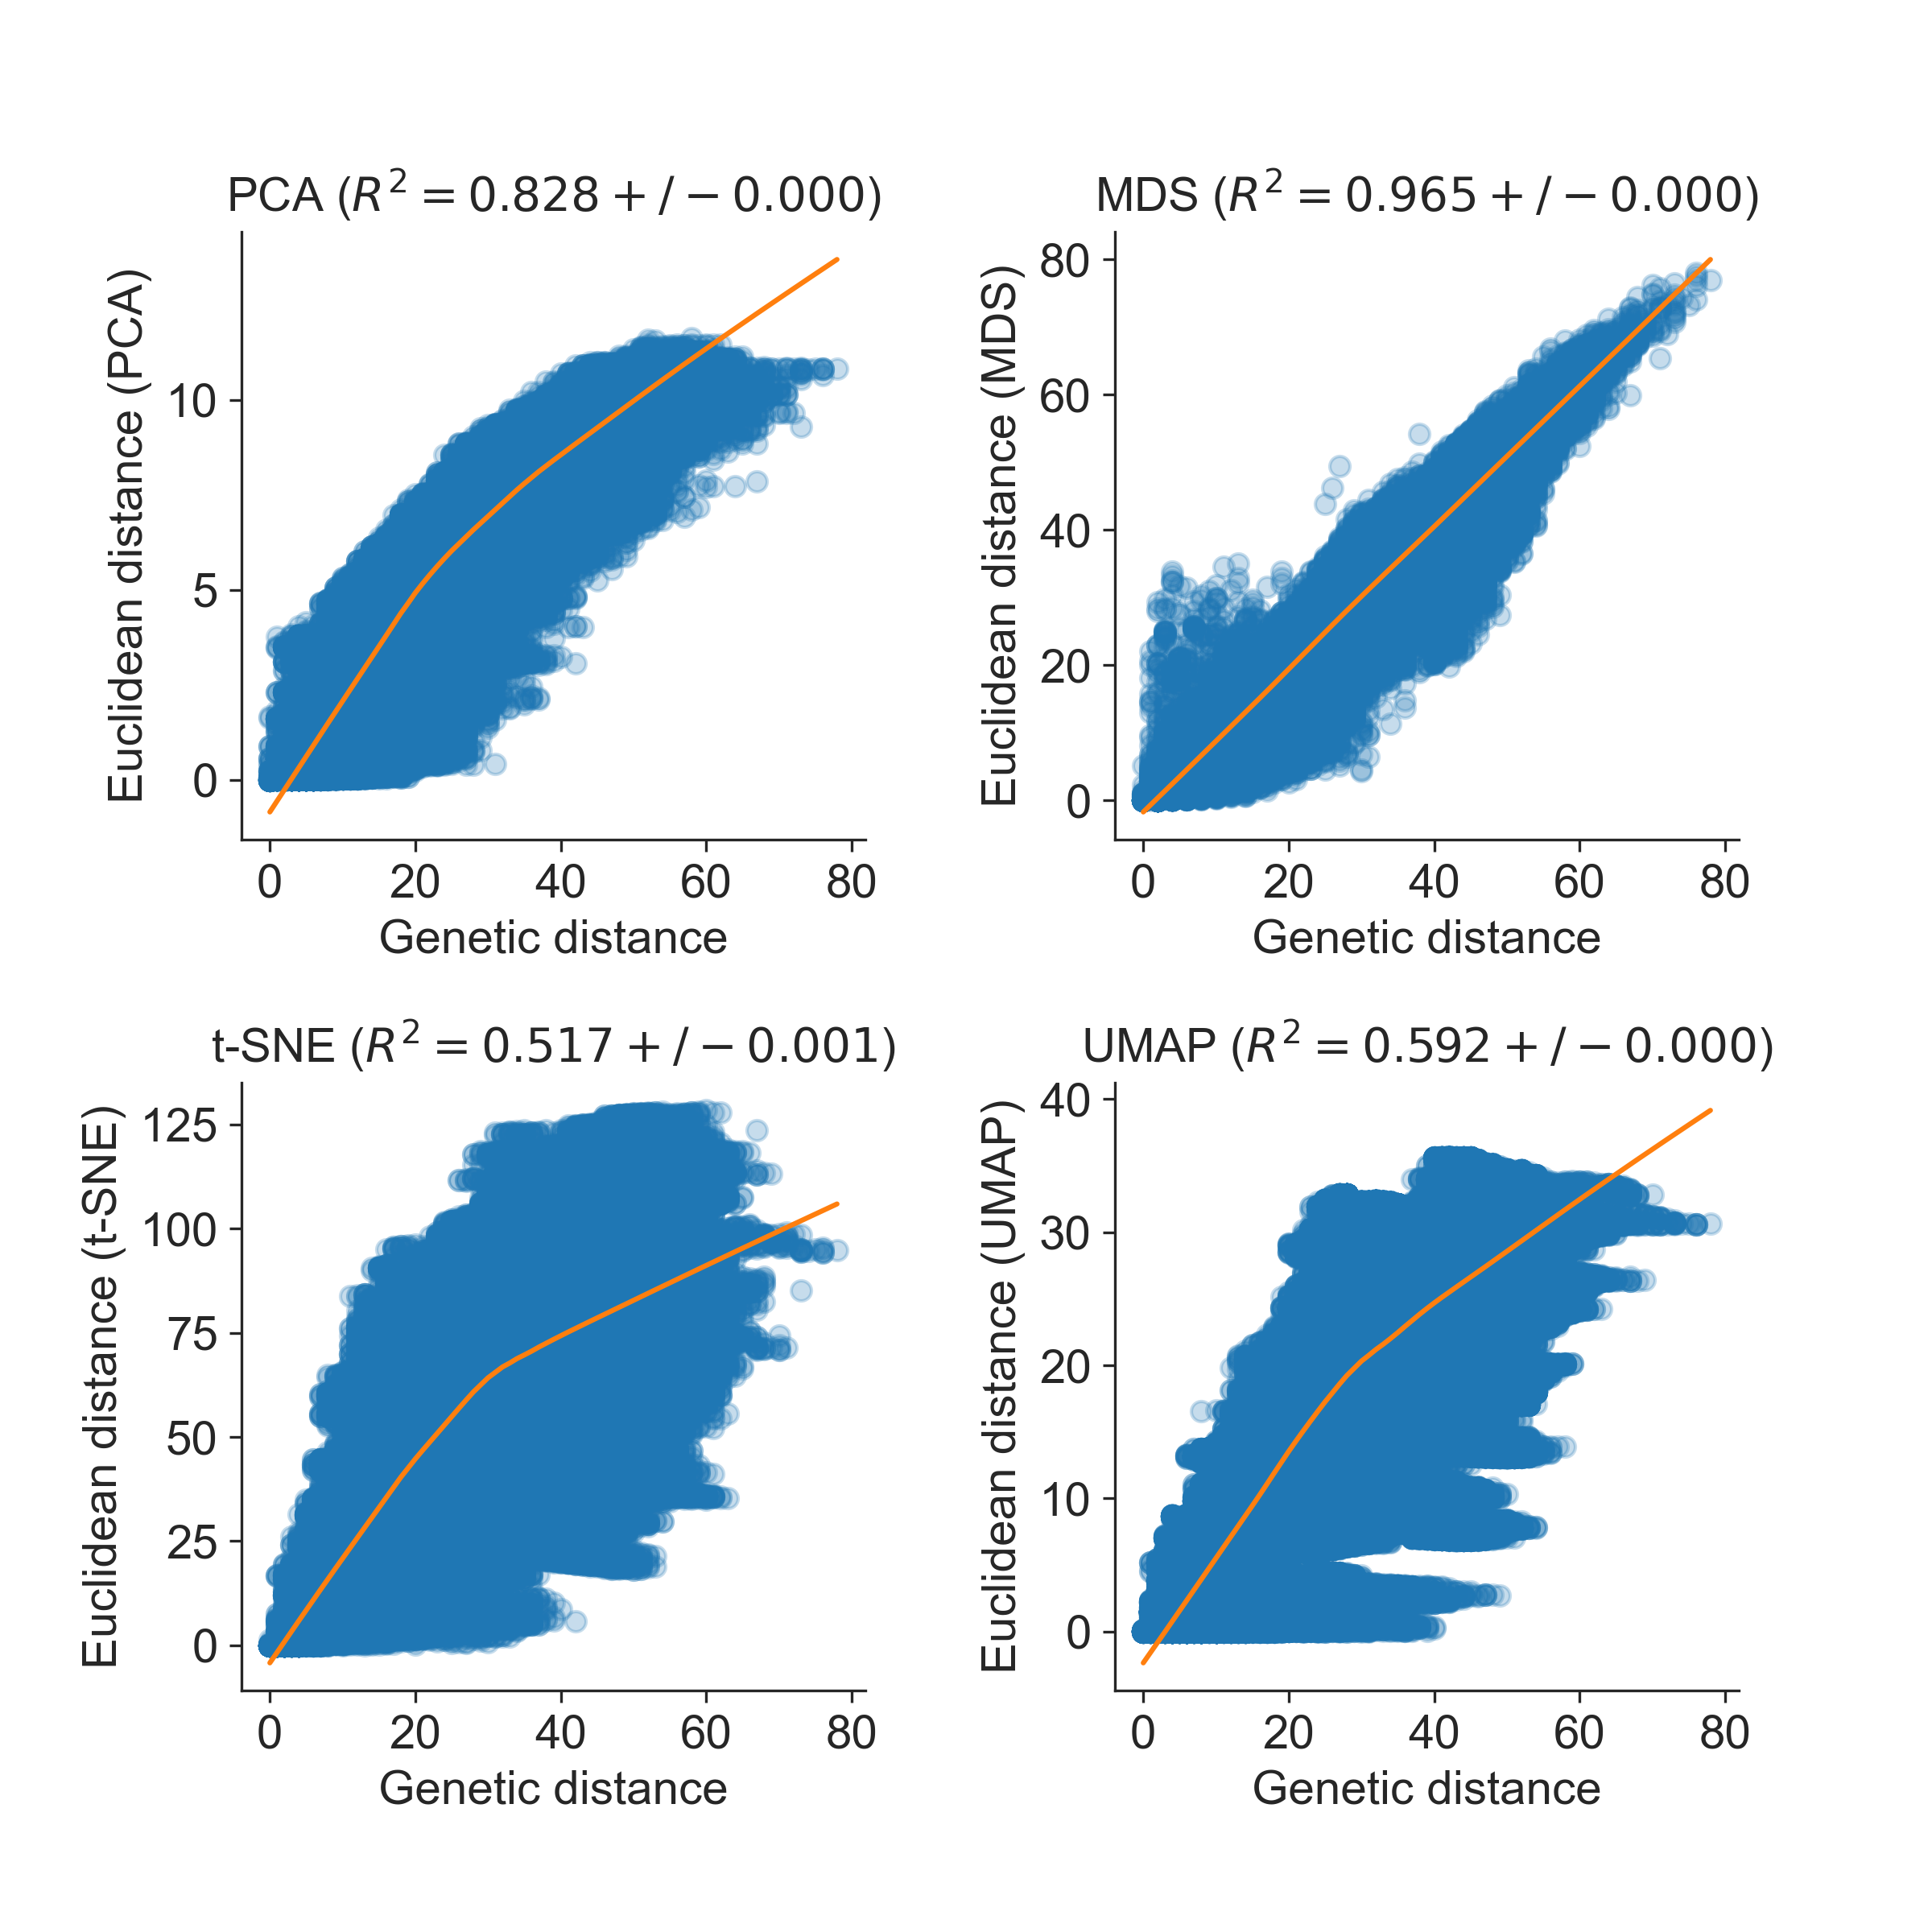
\includegraphics[width=\columnwidth]{figures/flu-2016-2018-ha-euclidean-distance-by-genetic-distance.png}
  \caption{
    The mapping between Euclidean and Genetic distance assess the strength of both the local and global structure of the embedding recapitulation.
    The scatterplot for PCA (upper left), MDS (upper right), t-SNE (lower left), and UMAP (lower right) consistently exhibit linear relationships for pairs of strains that differ by around 20 nucleotides.
  }
  \label{fig:seasonal-influenza-h3n2-ha-pairwise-distances}
  \end{center}
\end{figure}

Next, we measured how well clusters of genomes in a given embedding corresponded to our expert clade annotations.
For each embedding described above, we applied hierarchical clustering with HDBSCAN to assign cluster labels to each genome.
For each pair of genomes, we tested whether both genomes belonged to the same clade and the same cluster.
We calculated the accuracy of cluster labels using the Matthew's correlation coefficient (MCC) of the resulting pairwise tests \citep{matthews_1975}.
Since we previously identified the optimal HDBSCAN parameter based on this same accuracy metric and dataset, we anticipated that the cluster accuracy would be relatively high.
We counted genomes that HDBSCAN could not assign to a cluster as false negatives in our MCC calculation, but we also used this number of unassigned genomes as an additional metric of cluster quality.

As expected, the clusters for each method generally corresponded to larger phylogenetic clades (Figure~\ref{fig:seasonal-influenza-h3n2-ha-clusters}, Table~1).
The t-SNE embedding produced the most accurate classification (MCC = 0.756) with 20 clusters and \jhc{NNN} genomes not assigned to a cluster.
UMAP also accurately classified genomes (MCC = 0.662) with only five clusters and no unassigned genomes.
PCA (MCC = 0.368) and MDS (MCC = 0.476) both performed relatively poorly but for different reasons.
PCA combined genomes from divergent phylogenetic clades A1 and A2 into the same larger cluster (cluster 4) but managed to assign clusters to all but \jhc{NNN} genomes.
In contrast, MDS distinguished between most large clades including 3c3.A, A1, and A2, but it also placed closely-related strains from the same clades in two separate clusters (clusters 0 and 5) and failed to assign clusters to \jhc{NNN} genomes.
Clusters 0 and 5 correspond to the apparently arbitrary splitting of both clades A3 and A4 into different groups in MDS space described above.
These results indicate that nonlinear embeddings of t-SNE and UMAP could be better-suited for clustering and classification than linear embeddings from PCA and MDS.

\begin{figure}[htb]
  \begin{center}
  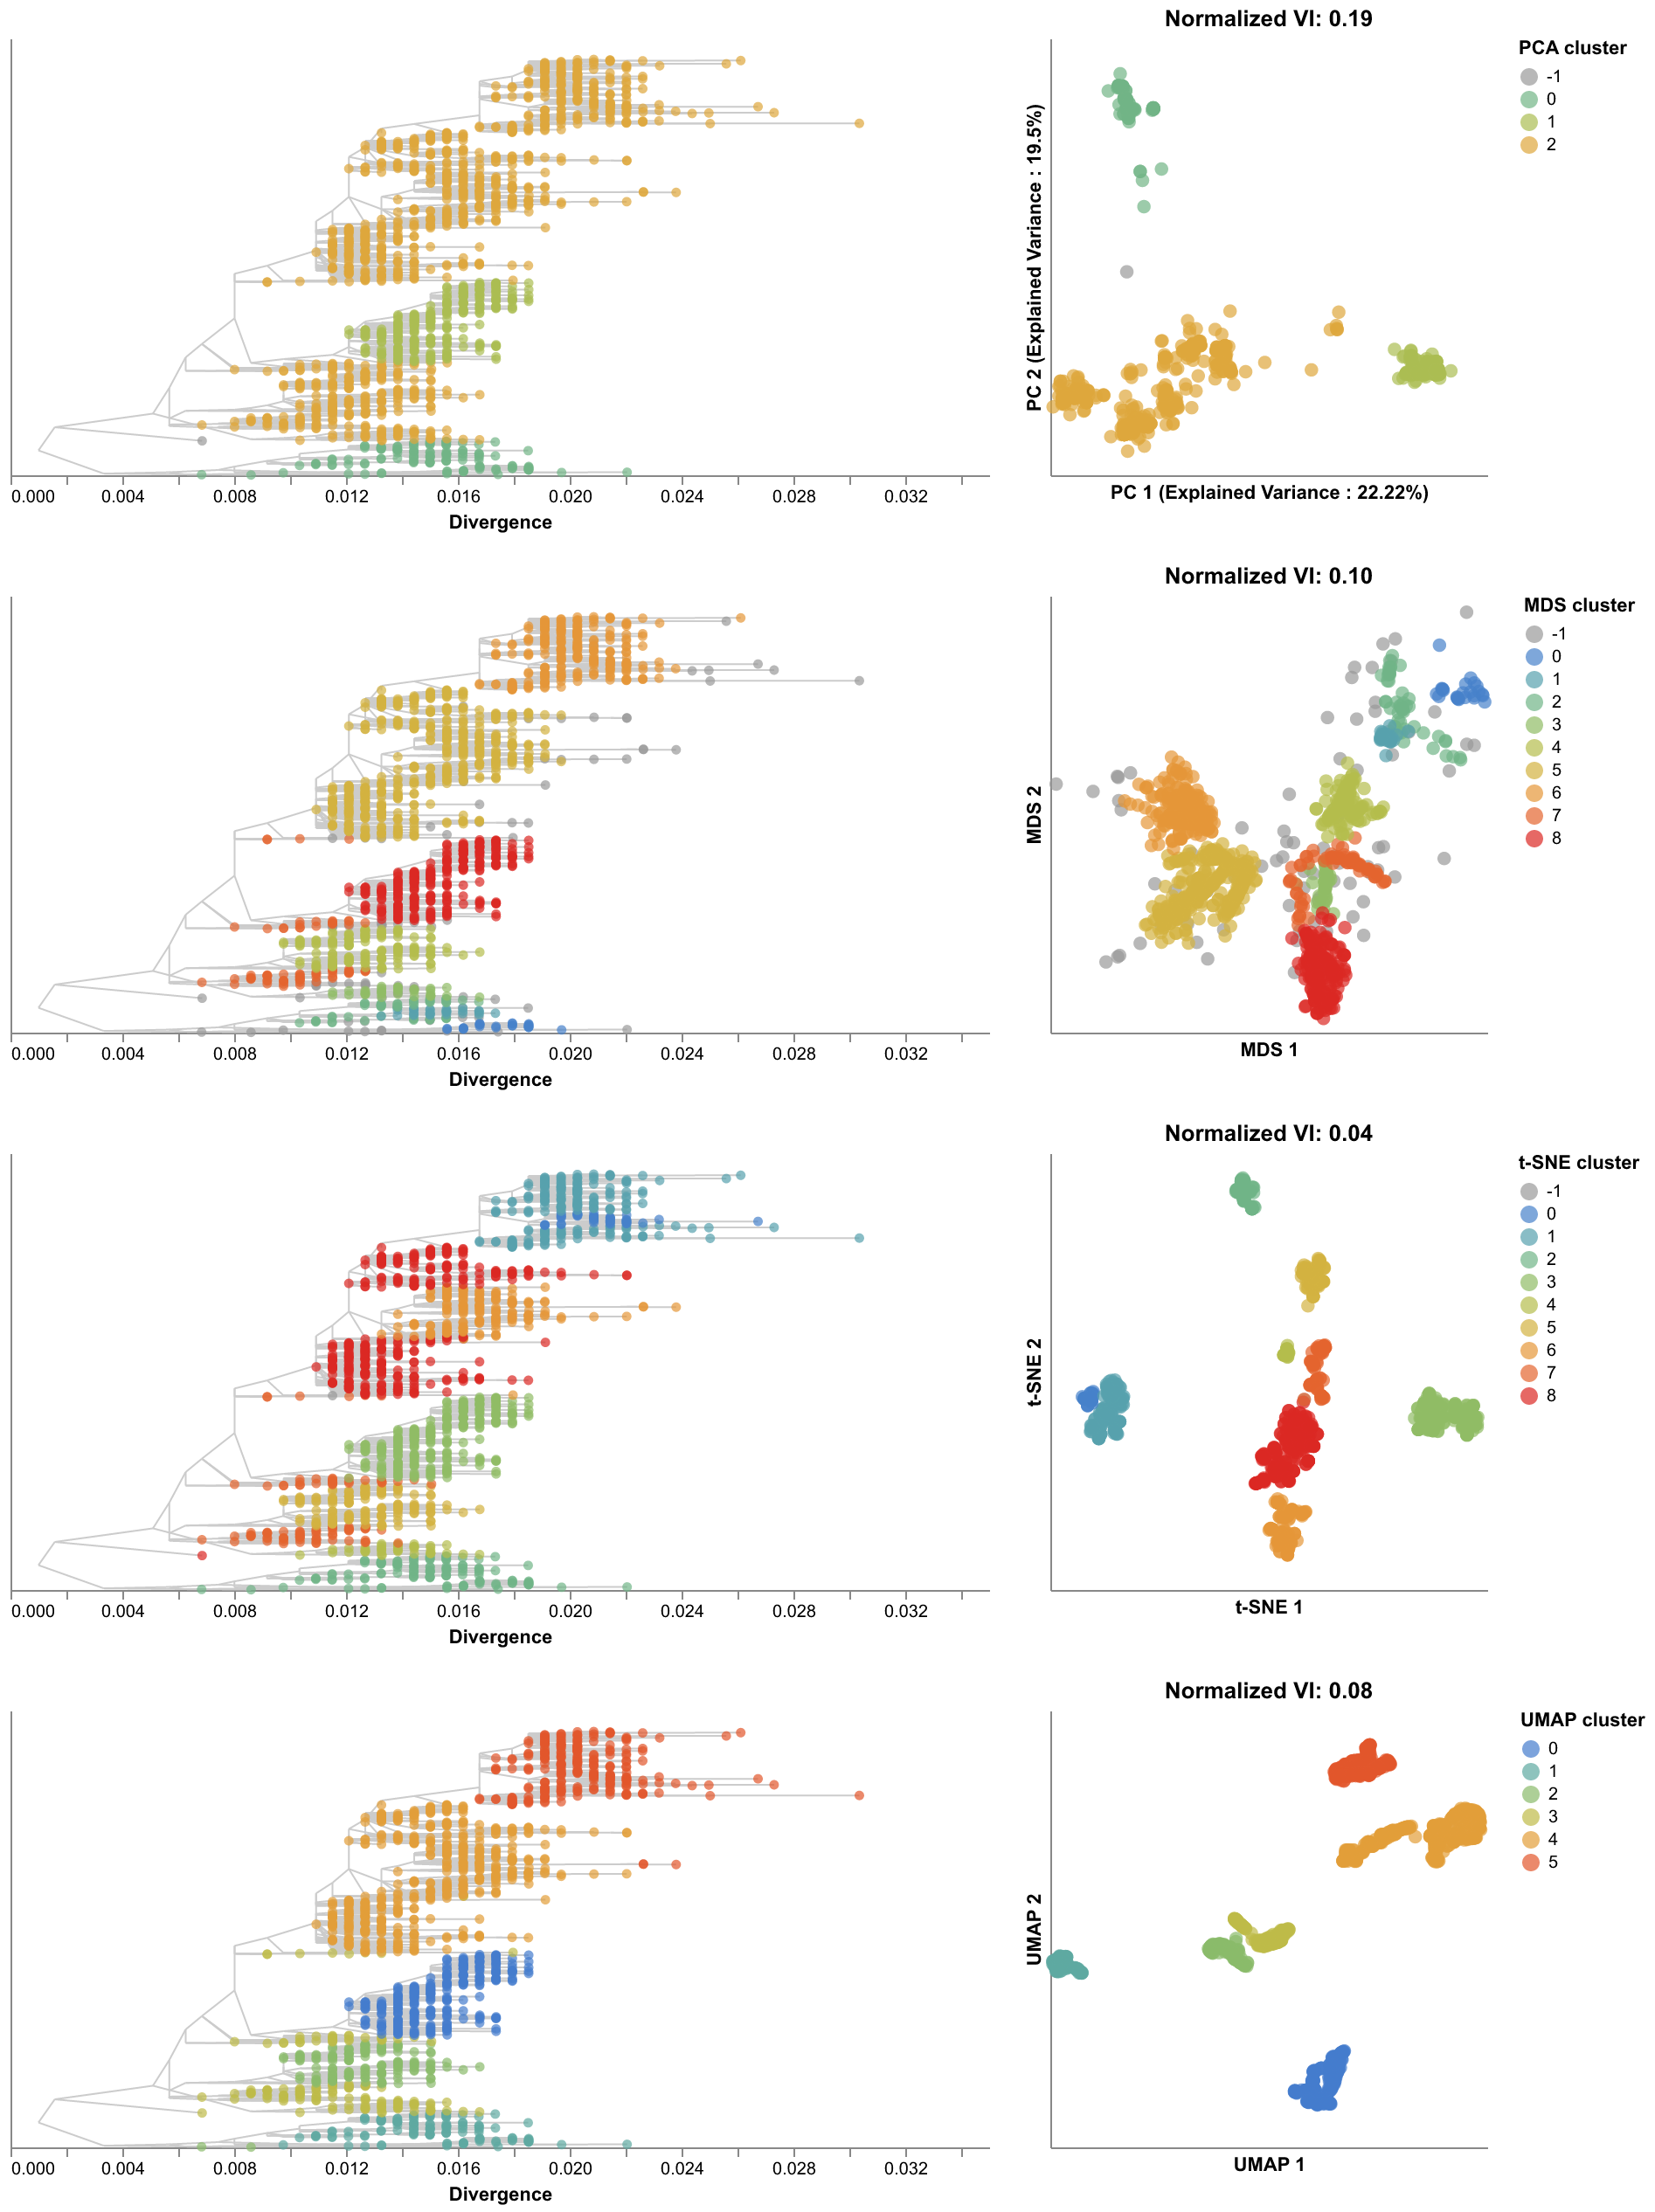
\includegraphics[width=\columnwidth]{figures/flu-2016-2018-ha-embeddings-by-cluster.png}
  \caption{
    The embeddings colored by their HDBSCAN label, with the distance threshold defined by the threshold that preserved the greatest amount of clade relationships.
    The chart for PCA (top left), MDS (middle left), t-SNE (middle left), and UMAP (bottom left) generally recapitulate groups of viruses into clades without inferring ancestral relationships, and the trees on the righthand side describes how these clade grouping appear on the tree, which does infer ancestral relations.
  }
  \label{fig:seasonal-influenza-h3n2-ha-clusters}
  \end{center}
\end{figure}

To understand whether these embedding methods could be used to cluster previously unseen genomes for the same virus, we applied each method to the test dataset spanning 2018--2020, clustered genomes in the embedding space with HDBSCAN, and calculated the accuracy of the cluster assignments based on previously defined clades.

\subsection*{Joint embeddings of hemagglutinin and neuraminidase genomes identify seasonal influenza virus A/H3N2 reassortment events}

\subsection*{MERS-CoV clusters correspond to host-specific outbreaks}

\subsection*{SARS-CoV-2 clusters recapitulate emerging lineage designations}

\section*{Discussion}

\section*{Materials and methods}

\subsection*{Hyperparameter optimization}

To test whether embeddings from each method could recapitulate phylogenetic clades, we performed a grid search of each method's parameter space during which we applied an embedding method to a randomly selected 50\% of the sequences in the multiple sequence alignment, identified clusters in the embedding with HDBSCAN \citep{hdbscan}, and calculated the accuracy of the cluster labels for each sequence compared to the known clade labels (see methods).
We used the resulting classification accuracies to identify the optimal distance threshold for HDBSCAN.
We fixed the HDBSCAN threshold to its optimal value and repeated the same procedure on the other 50\% of the sequences.
We used the resulting accuracies to identify the optimal t-SNE and UMAP parameters.
Finally, we applied each embedding method to the full training dataset with the optimal method parameters, clustered the embeddings with HDBSCAN's optimal distance threshold, and evaluated the accuracy of the cluster classifications.

\subsection*{Data and software availability}

The entire workflow for our analyses was implemented with Snakemake \citep{molder_2021}.
We have provided all source code, configuration files, and datasets at \href{https://github.com/blab/cartography}{https://github.com/blab/cartography}.

\section*{Acknowledgments}

\section*{Author contributions}

SN...
JH...
AB...
TB...

\section*{Competing interests}

The authors declare that no competing interests exist.

\section*{Supplemental Files}

\bibliography{cartography}

\end{document}
